\documentclass[conference]{IEEEtran}
\IEEEoverridecommandlockouts
% The preceding line is only needed to identify funding in the first footnote. If that is unneeded, please comment it out.
\usepackage{cite}
\usepackage{dblfloatfix}
\usepackage{amsmath,amssymb,amsfonts}
\usepackage{algorithmic}
\usepackage{listings}
\usepackage{graphicx}
\usepackage{textcomp}
\usepackage{xcolor}
\def\BibTeX{{\rm B\kern-.05em{\sc i\kern-.025em b}\kern-.08em
    T\kern-.1667em\lower.7ex\hbox{E}\kern-.125emX}}
\begin{document}

\title{Implementing K-Nearest Neighbors (KNN)\\
}

\author{\IEEEauthorblockN{Devopriya Tirtho}
\IEEEauthorblockN{16.02.04.033}
\IEEEauthorblockA{\textit{Department of Computer Science and Engineering} \\
\textit{Ahsanullah University of Science and Technology}\\
Dhaka, Bangladesh \\
}

}

\maketitle

\begin{abstract}
In \textbf{'Machine Learning'}, for predicting the accurate class of an unknown sample we need to visualize our training samples whether they are linearly separable or not. \textbf{K-Nearest Neighbors'} classifier helps to classify data points perfectly with the help of euclidean distance between points and classify them according to nearest neighbors. This classifier is a robust model for classifying unknown data points with the help of trained data.
\end{abstract}

\begin{IEEEkeywords}
Machine Learning, K-Nearest Neighbors, Euclidean Distance, Neighbor.
\end{IEEEkeywords}

\section{Introduction}
\textbf{K-Nearest Neighbors} is also known as \textbf{KNN} classifier. This type of classifier is used for regression and classification problem. For the both types, this method works with the help of \textbf{K} numbered nearest neighbors. For classification, from a supervised dataset the data points are defined properly. For unknown samples, each sample is measured by the distance from the point to each of the training points. After distance measurement, the K-nearest neighbors are picked and the type of class which is in majority define the sample point's class. The main drawback of the classification method is picking the \textbf{K} number and problem occurs when the class distribution is skewed. Here, in this assignment, we will implement a \textbf{K-Nearest Neighbors} classifier to predict the class of some unknown samples.

\section{Task}

There are two datasets named 'train' and 'test' where all the datapoints are given. The 'train' dataset is provided with datapoints along with their respective classes. The 'train' datapoints with their respective classes are given :\\
\begin{table}[htbp]
\caption{Table for Sample Training Data}
\begin{center}
\begin{tabular}{|c|c|c|}
\hline
\textbf{\textit{X1}}&\textbf{\textit{X2}}& \textbf{\textit{Class}} \\
\hline
\textbf{{7}}&\textbf{{7}}&   \textbf{{1}} \\
\hline
\textbf{{7}}&\textbf{{4}}&   \textbf{{1}} \\
\hline
\textbf{{6}}&\textbf{{4}}&   \textbf{{1}} \\
\hline
\textbf{{7}}&\textbf{{5}}&   \textbf{{1}} \\
\hline
\textbf{{7}}&\textbf{{6}}&   \textbf{{1}} \\
\hline
\textbf{{6}}&\textbf{{7}}&   \textbf{{1}} \\
\hline
\textbf{{6}}&\textbf{{6}}&   \textbf{{1}} \\
\hline
\textbf{{3}}&\textbf{{4}}&   \textbf{{2}} \\
\hline
\textbf{{2}}&\textbf{{3}}&   \textbf{{2}} \\
\hline
\textbf{{3}}&\textbf{{2}}&   \textbf{{2}} \\
\hline
\textbf{{4}}&\textbf{{3}}&   \textbf{{2}} \\
\hline
\textbf{{3}}&\textbf{{3}}&   \textbf{{2}} \\
\hline
\textbf{{4}}&\textbf{{4}}&   \textbf{{2}} \\
\hline
\textbf{{1}}&\textbf{{4}}&   \textbf{{2}} \\
\hline
\end{tabular}
\label{tab1}
\end{center}
\end{table}

Then there is a 'test' dataset which is given with the datapoints to predict the accurate classes of those samples. The 'test' datapoints are given below:\\
$W$= $\{(3,7),(7,7),(4,3),(2,8),(3,5),(1,2),(4,8),(8,3),(8,4)\}$\\

Here are the tasks, which we have to do for implementing the \textbf{K-Nearest Neighbors} classifier:
\begin{itemize}  
\item The first task is to take input from the 'train' dataset and plot them with different colored markers according to the assigned class label.
\item Then, we have to implement the \textbf{KNN} algorithm where the value of 'K' has to be taken from the user.
\item Finally, we have to print the top 'K' distances along with their class labels.

\end{itemize}
\section{Experimental Design}
\begin{itemize}  
\item For the first task, we have to plot the datapoints with according to their class labels with different colored markers. 
\begin{figure}[htb!]
\centerline{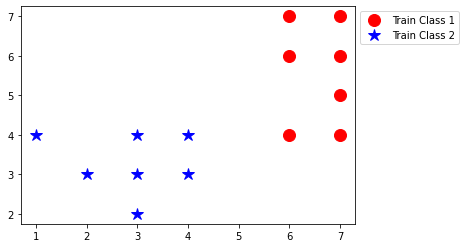
\includegraphics[scale=0.5]{41.png}}
\caption{Visualization of the Training Samples\\}
\label{fig}
\end{figure}
\item For the implementation of the \textbf{K-Nearest Neighbors} classifier, we need to take each datapoint and find the \textbf{Euclidean Distance} from each training samples. The rule for calculating the \textbf{Euclidean Distance} is:\\
\begin{equation}
\sqrt{\left(x_{2}-x_{1}\right)^{2}+\left(y_{2}-y_{1}\right)^{2}}
\end{equation}
\item Then, we have to take input of 'K' and find the K-nearest neighbors to classify the datapoint. Here, is a example of predicting the class of $(3,7)$ datapoint in a tabular form:\\
\begin{table}[htbp]
\begin{tabular}{llllll}
\hline
\multicolumn{1}{c}{X1} & \multicolumn{1}{c}{X2} & \multicolumn{1}{c}{\begin{tabular}[c]{@{}c@{}}Squared Distance \\ to\\ (3,7)\end{tabular}} & \begin{tabular}[c]{@{}l@{}}Rank \\ Minimum \\ Distance\end{tabular} & \multicolumn{1}{c}{\begin{tabular}[c]{@{}c@{}}K=3, is \\ it included?\end{tabular}} & Class \\
\hline
7                      & 7                      & (7-3)\textasciicircum{}2+(7-7)\textasciicircum{}2
=
&16                                                                  & No                                                                                  & N/A   \\
\hline
7                      & 4                      & (7-3)\textasciicircum{}2+(4-7)\textasciicircum{}2                                         = & 25                                                                  & No                                                                                  & N/A   \\
\hline
6                      & 4                      & (6-3)\textasciicircum{}2+(4-7)\textasciicircum{}2                                         = & 18                                                                  & No                                                                                  & N/A   \\
\hline
7                      & 5                      & (7-3)\textasciicircum{}2+(5-7)\textasciicircum{}2                                         = & 20                                                                  & No                                                                                  & N/A   \\
\hline
7                      & 6                      & (7-3)\textasciicircum{}2+(6-7)\textasciicircum{}2                                         = & 17                                                                  & No                                                                                  & N/A   \\
\hline
6                      & 7                      & (6-3)\textasciicircum{}2+(7-7)\textasciicircum{}2                                         = & 9                                                                   & Yes                                                                                 & 1     \\
\hline
6                      & 6                      & (6-3)\textasciicircum{}2+(6-7)\textasciicircum{}2                                         = & 10                                                                  & Yes                                                                                 & 1     \\
\hline
3                      & 4                      & (3-3)\textasciicircum{}2+(4-7)\textasciicircum{}2                                         = & 9                                                                   & Yes                                                                                 & 2     \\
\hline
2                      & 3                      & (2-3)\textasciicircum{}2+(3-7)\textasciicircum{}2                                         = & 17                                                                  & No                                                                                  & N/A   \\
\hline
3                      & 2                      & (3-3)\textasciicircum{}2+(2-7)\textasciicircum{}2                                         = & 25                                                                  & No                                                                                  & N/A   \\
\hline
4                      & 3                      & (4-3)\textasciicircum{}2+(3-7)\textasciicircum{}2                                         = & 17                                                                  & No                                                                                  & N/A   \\
\hline
3                      & 3                      & (3-3)\textasciicircum{}2+(3-7)\textasciicircum{}2                                         = & 16                                                                  & No                                                                                  & N/A   \\
\hline
4                      & 4                      & (4-3)\textasciicircum{}2+(4-7)\textasciicircum{}2                                         = & 10                                                                  & No                                                                                  & N/A   \\
\hline
1                      & 4                      & (1-3)\textasciicircum{}2+(4-7)\textasciicircum{}2                                         = & 13                                                                  & No                                                                                  & N/A  \\
\hline
\end{tabular}
\end{table}
\\
Here, the predicted class is $1$ as the majority of nearest neighbors refer to class $1$.\\

\item Finally, we have printed the class labels for each datapoint with the stat. \\
\begin{figure}[htb!]
\centerline{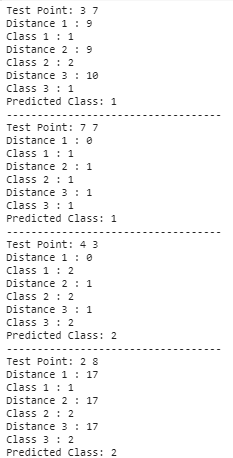
\includegraphics[scale=0.9]{43.png}}
\caption{Output of Test Samples after Implementing KNN Algorithm\\}
\label{fig}
\end{figure}
\end{itemize}

\section{Result Analysis}
The classification for sample data is given below:
\begin{table}[htbp]
\caption{Table for Classification of Sample Data}
\begin{center}
\begin{tabular}{|c|c|c|}
\hline
\textbf{\textit{X1}}&\textbf{\textit{X2}}& \textbf{\textit{Class}} \\
\hline
\textbf{{3}}&\textbf{{7}}&   \textbf{{1}} \\
\hline
\textbf{{7}}&\textbf{{7}}&   \textbf{{1}} \\
\hline
\textbf{{4}}&\textbf{{3}}&   \textbf{{2}} \\
\hline
\textbf{{2}}&\textbf{{8}}&   \textbf{{2}} \\
\hline
\textbf{{3}}&\textbf{{5}}&   \textbf{{2}} \\
\hline
\textbf{{1}}&\textbf{{2}}&   \textbf{{2}} \\
\hline
\textbf{{4}}&\textbf{{8}}&   \textbf{{1}} \\
\hline
\textbf{{8}}&\textbf{{3}}&   \textbf{{1}} \\
\hline
\textbf{{8}}&\textbf{{4}}&   \textbf{{1}} \\
\hline

\end{tabular}
\label{tab1}
\end{center}
\end{table}
\begin{figure}[htb!]
\centerline{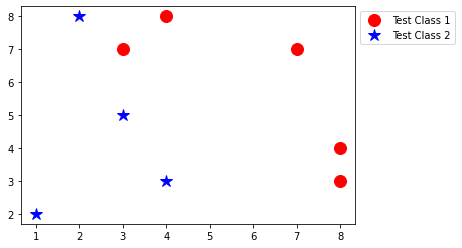
\includegraphics[scale=0.5]{42.png}}
\caption{Visualization of Testing Data\\}
\label{fig}
\end{figure}
\section{Python Code}



\begin{lstlisting}
# -*- coding: utf-8 -*-
"""160204033_Assignment04.ipynb

Automatically generated by Colaboratory.

Original file is located at
    https://colab.research.google.com/
drive/1IIedNgjzpWxBnt-J25YWg75iCnJ2J5nr
"""

import pandas as pd 

import numpy as np
import matplotlib.pyplot as plt 

train_data = pd.read_csv('train_knn.txt', 
sep=",", header=None) 
train_data.columns = ["x1", "y1","class"]

train_data

test_data = pd.read_csv('test_knn.txt',
 sep=",", header=None)  
test_data.columns = ["x1", "y1"] 

test_data

b=train_data.shape 
print(b[0]) 
RowNumber=b[0] 

c=test_data.shape 
print(c[0]) 
RowNumberTest=c[0] 

train_class1_x=[]
train_class1_y=[]
train_class2_x=[]
train_class2_y=[]


for i in range(0,RowNumber):
    y=train_data.at[i,'class']
    if(y==1):
      train_class1_x.
	append(train_data.at[i,'x1'])
      train_class1_y.
	append(train_data.at[i,'y1'])
    else:
      train_class2_x.
	append(train_data.at[i,'x1'])
      train_class2_y.
	append(train_data.at[i,'y1'])


plt.plot(train_class1_x,train_class1_y, 
'ro', markersize=12,label="Train Class 1")
plt.plot(train_class2_x,train_class2_y,
'b*', markersize=12,label="Train Class 2")
plt.legend(bbox_to_anchor=(1, 1),
 loc="upper left")

NearestNeighbor=3


class_predict=[]
class_final_predict=[]
distance=[]
for i in range(0,RowNumberTest): 
  print("Test Point:",
  test_data.at[i,'x1'],
  test_data.at[i,'y1'])
  for j in range(0,RowNumber):   
      distance_cal=(train_data.at[j,'x1']-
	test_data.at[i,'x1'])**2 + 
      (train_data.at[j,'y1']-
	test_data.at[i,'y1']) **2
      class_pred=train_data.at[j,'class']
      distance.
	append([distance_cal,class_pred])
  distance.sort() 
  for k in range(0,NearestNeighbor):
  
  dis_array=np.array(distance)
  
  for k in range (0, NearestNeighbor):
    print("Distance",k+1,":",dis_array[k,0])
    print("Class",k+1,":",dis_array[k,1])
    class_predict.append(dis_array[k,1])


  class1=class_predict.count(1)
  class2=class_predict.count(2)
  if (class1>class2):
    class_final_predict.append(1)
    print("Predicted Class: 1",)
  else:
    class_final_predict.append(2)
    print("Predicted Class: 2",)

  print("-----------------------------------")  
  class_predict=[]
  distance=[]


print(class_final_predict)

test_data['class']=class_final_predict

test_data

test_class1_x=[]
test_class1_y=[]
test_class2_x=[]
test_class2_y=[]


for i in range(0,RowNumberTest):
    y=test_data.at[i,'class']
    if(y==1):
      test_class1_x.
	append(test_data.at[i,'x1'])
      test_class1_y.
	append(test_data.at[i,'y1'])
    else:
      test_class2_x.
	append(test_data.at[i,'x1'])
      test_class2_y.
	append(test_data.at[i,'y1'])


plt.plot(test_class1_x,test_class1_y,
'ro', markersize=12,label="Test Class 1")
plt.plot(test_class2_x,test_class2_y, 
'b*', markersize=12,label="Test Class 2")
plt.legend(bbox_to_anchor=(1, 1),
 loc="upper left")


\end{lstlisting}


\section{Conclusion}

\textbf{‘KNN Classifier’} is a simple classification technique which uses \textbf{Euclidean Distancing} method to classify sample points according to number of nearest neighbors. 




\end{document}
